\part{Efekty}

\section{Prototyp urządzenia}
Finalna wersja urządzenia została zmontowana na płytce prototypowej. (Rysunek \ref{fig:device})
Z przodu urządzenia widoczny jest wyświetlacz LCD i ceramiczna antena modułu GPS, z tyłu znajdują się mikrokontrolej na płytce prototypowej, moduł GPS i moduł magnetometru.
Prototyp korzysta z zasilania zewnętrznego poprzez kabel USB.

\begin{figure}[h]
    \centering
    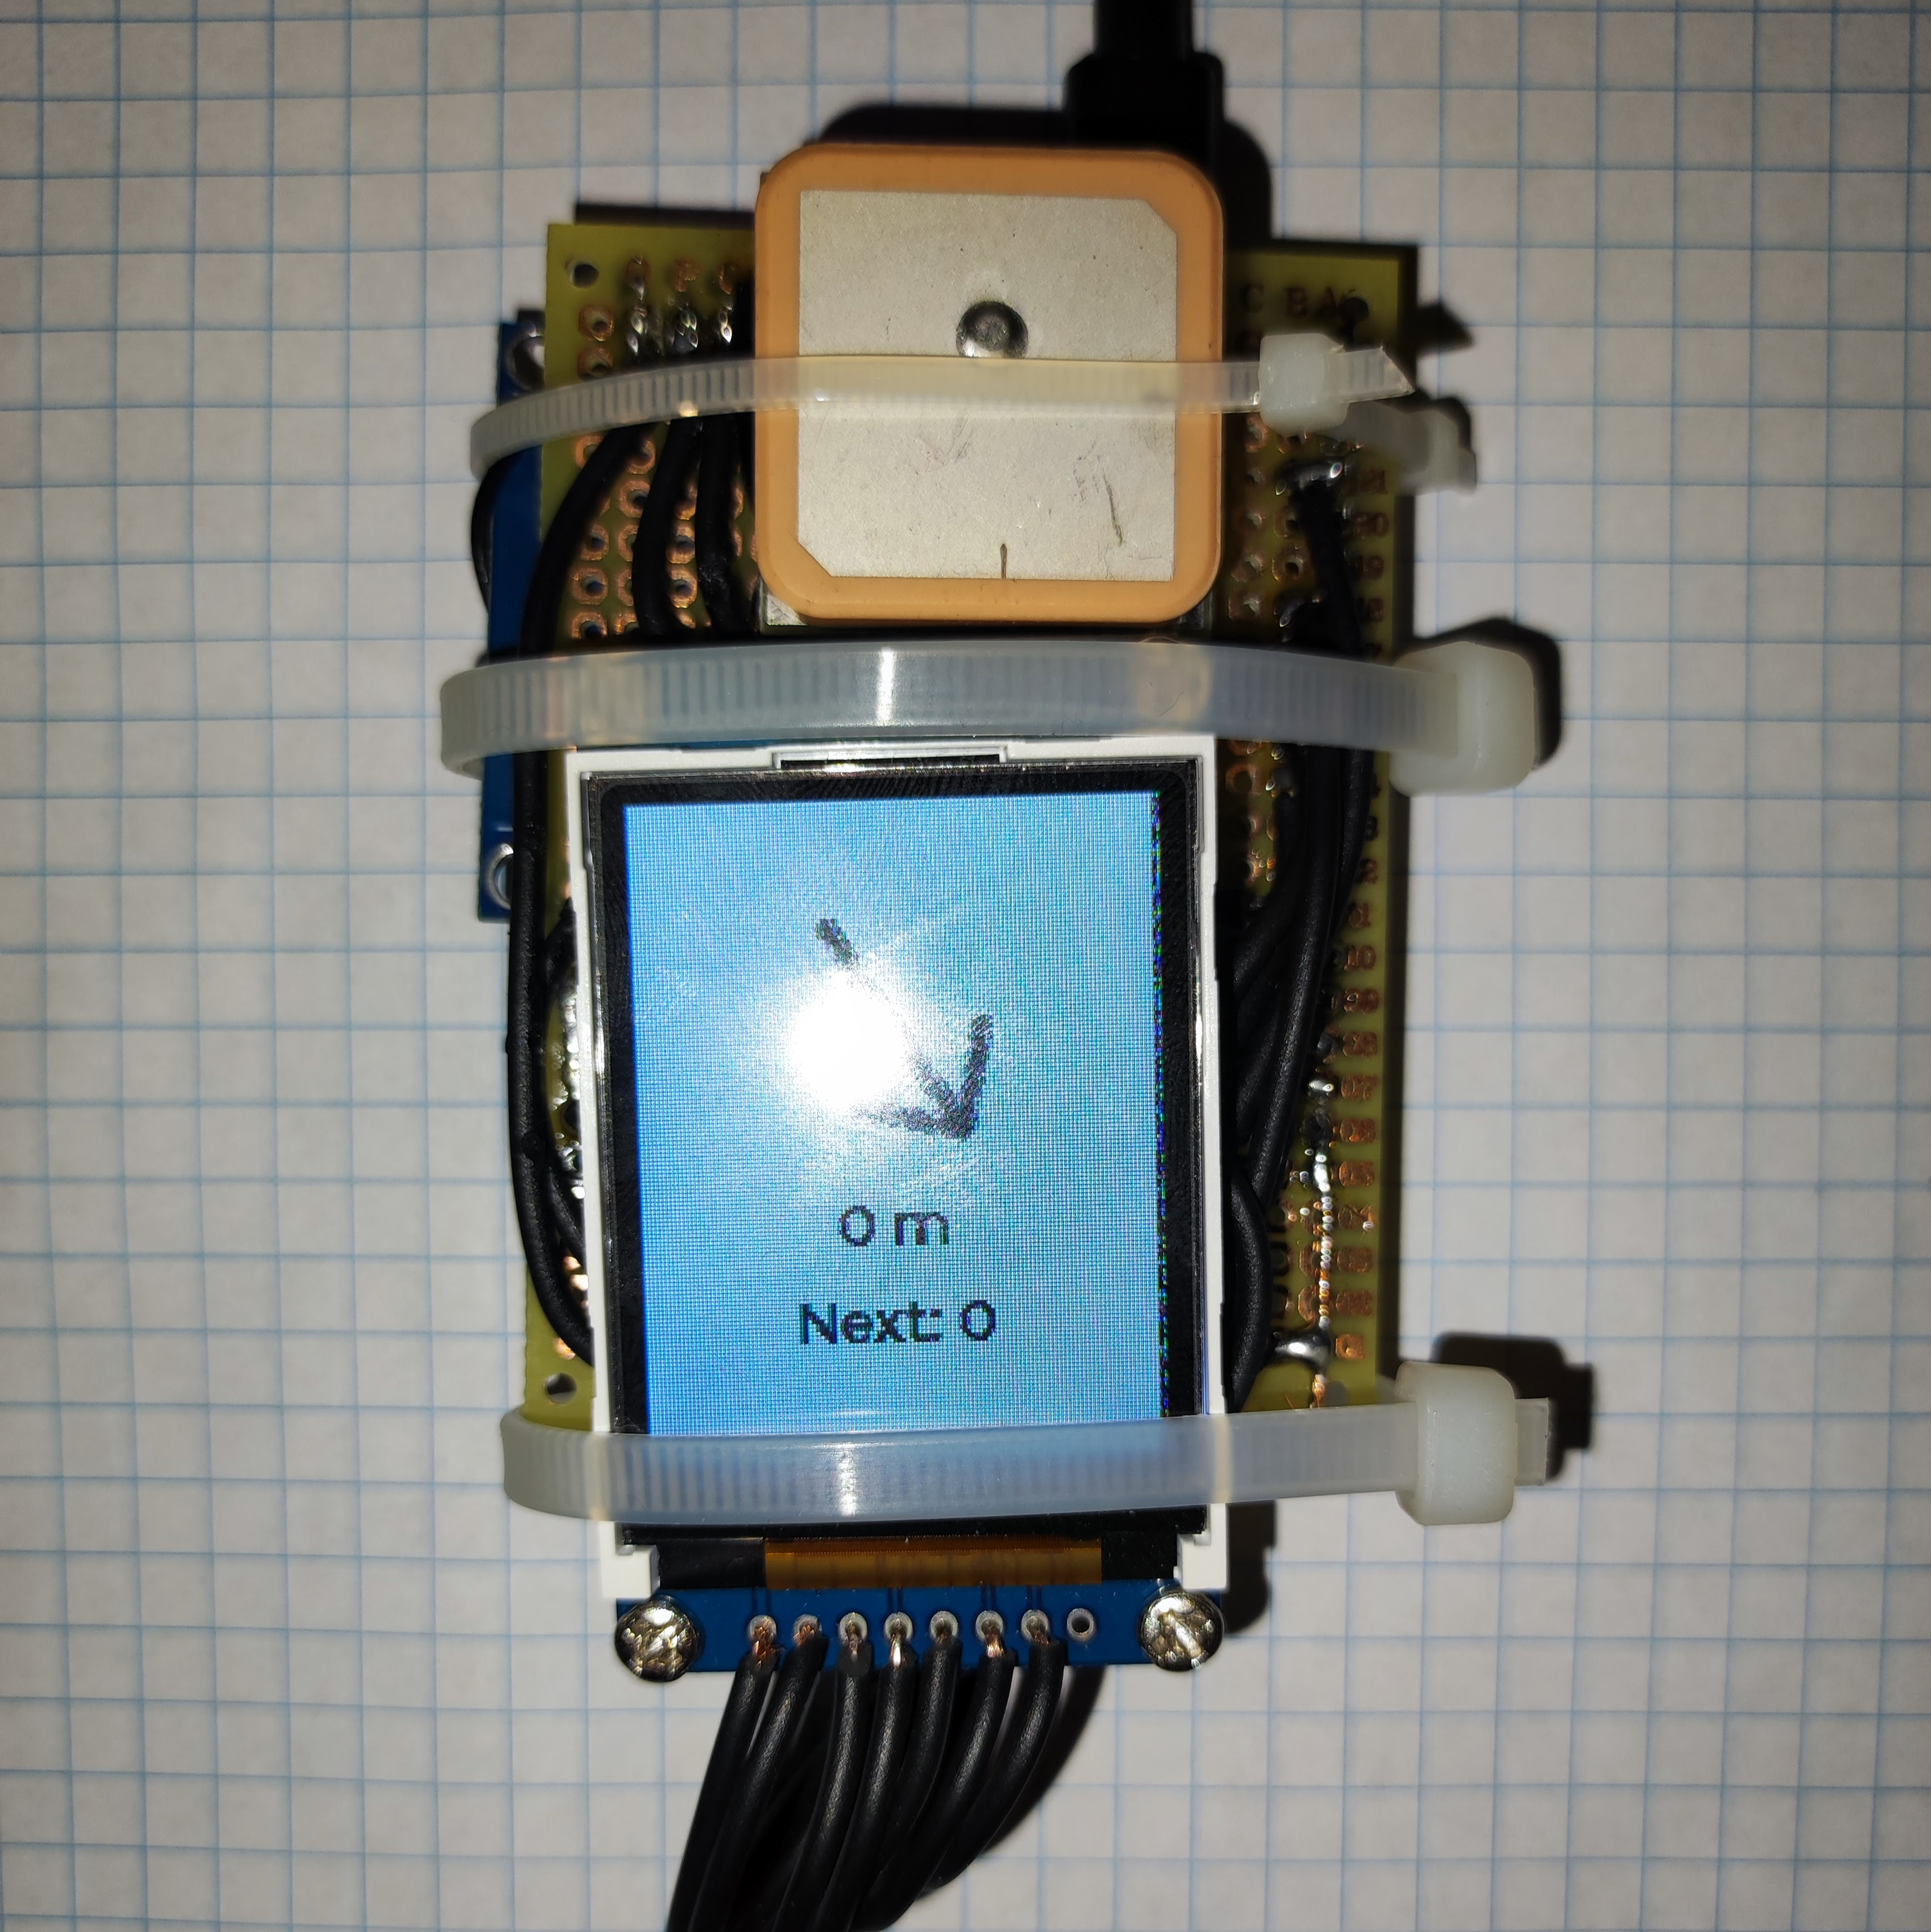
\includegraphics[width=0.4\textwidth]{res/front.jpg}
    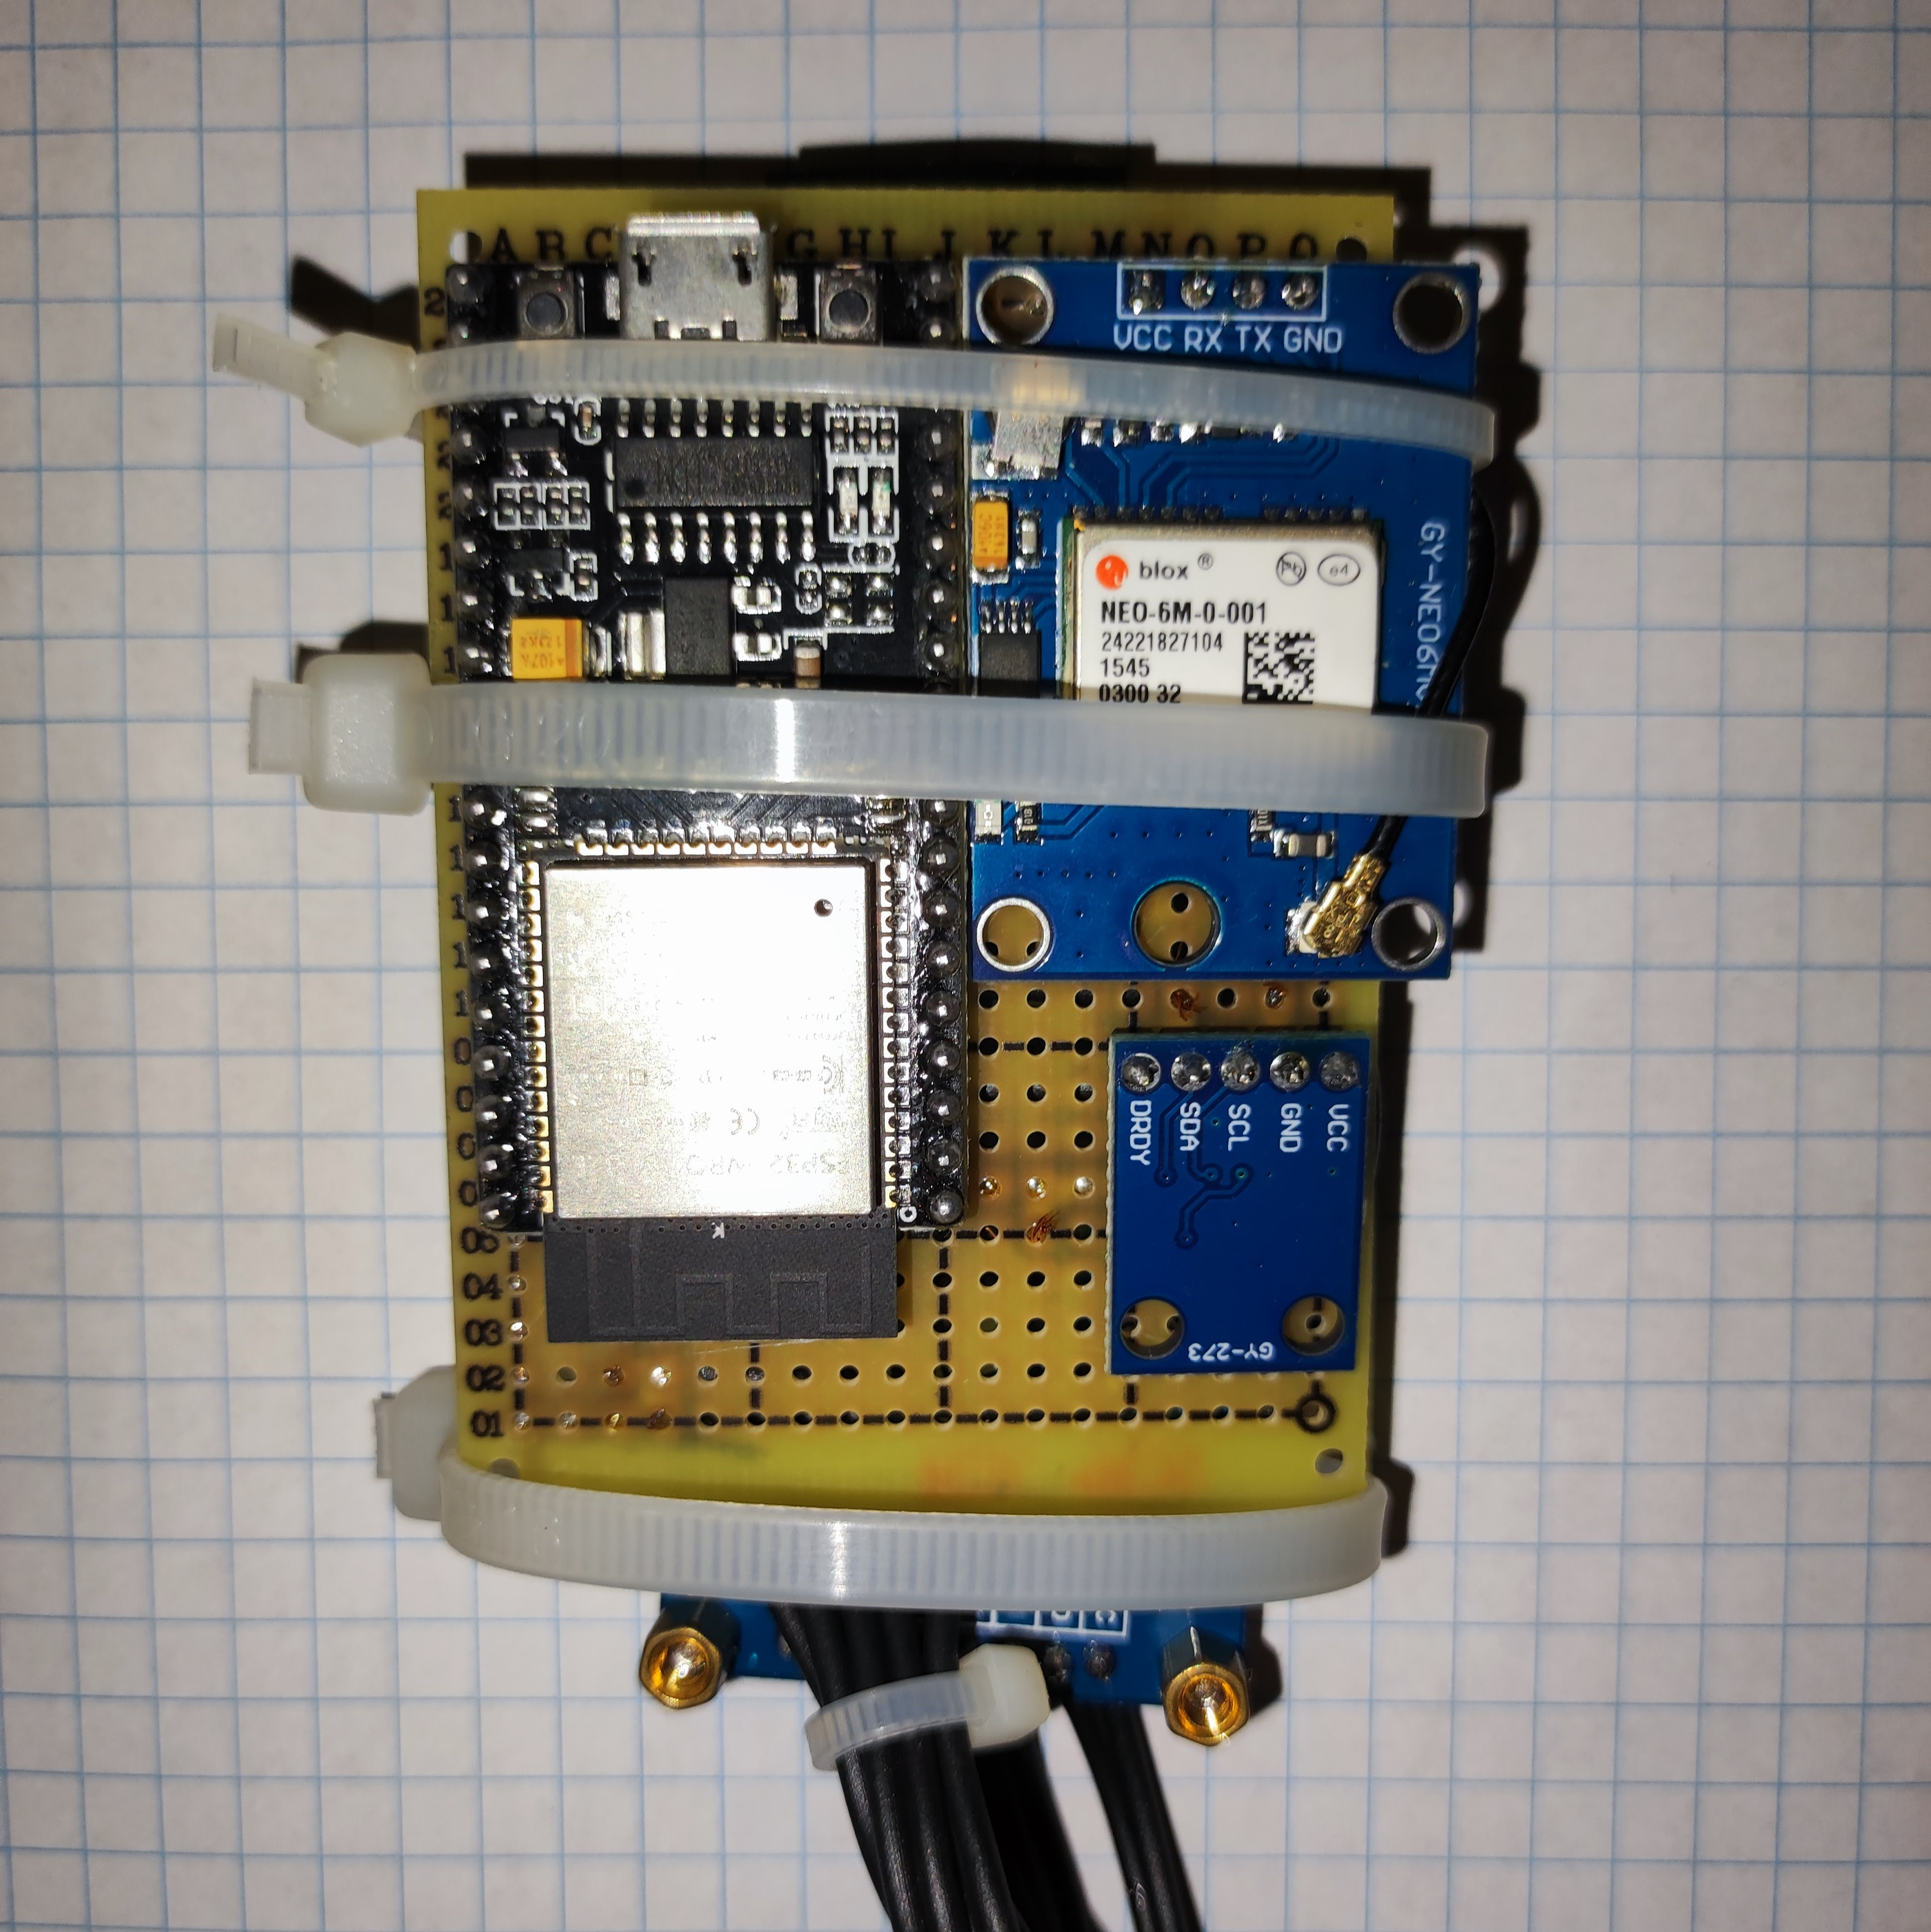
\includegraphics[width=0.4\textwidth]{res/back.jpg}
    \caption{Prototyp urządzenia (widok z przodu i z tyłu)}
    \label{fig:device}
\end{figure}

\subsection{Funkcjonalności}
W aktualnej wersji urządzenie jest w stanie:
\begin{itemize}
    \item Odczytywać dane z modułu GPS i magnetometru.
    \item Nawiązać połączenie w trybie BLE z aplikacją mobilną.
    \item Odbierać komendy od aplikacji mobilnej. (dane o nowej trasie)
    \item Wyświetlać na ekranie informacje o:
          \begin{itemize}
              \item Numerze następnego punktu na trasie
              \item Kierunku do następnego punktu
              \item Odległości do następnego punktu
              \item Zakończeniu nawigacji
          \end{itemize}
\end{itemize}

\section{Aplikacja mobilna}
\subsection{Widoki aplikacji}
\subsubsection{BLE connection}

\begin{figure}[H]
    \centering
    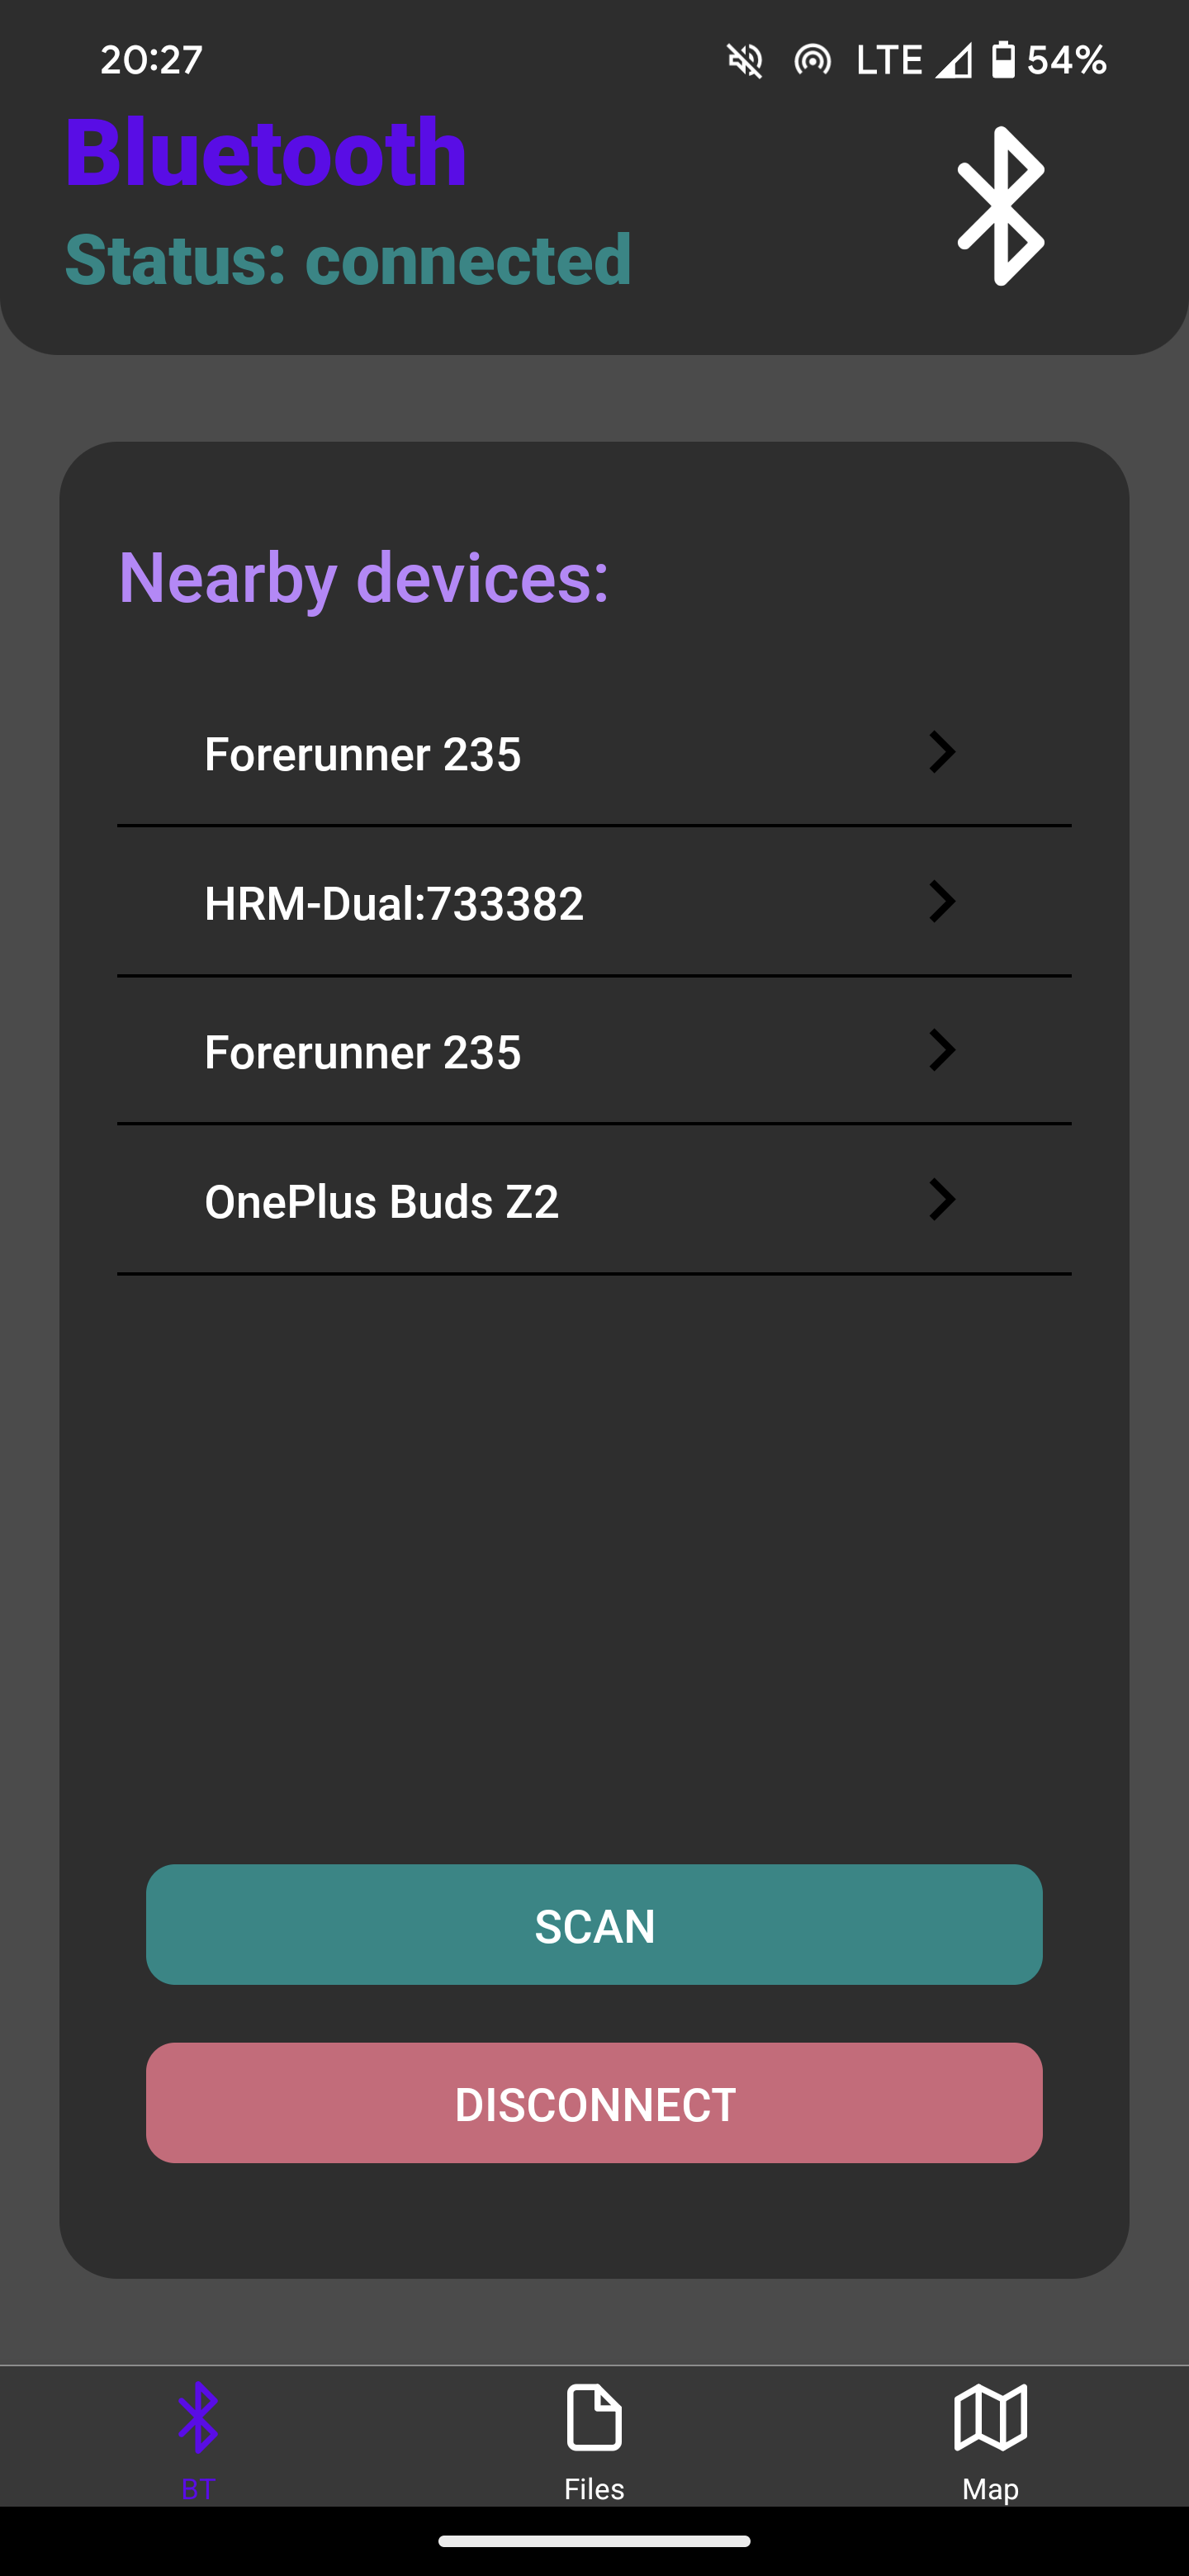
\includegraphics[scale = 0.07]{res/BT.png}
    \caption{Ekran BLE connection}
\end{figure}

Widok ten pozwala użytkownikowi rozpocząć skanowanie pobliskich urządzeń BLE, a następnie wybrać jedno z nich i połączyć się z nim. Jeśli jest to urządzenie SmartCompass, to znaleziony zostanie udostępniany przez nie serwis BLE, którego UUID zapisane jest w aplikacji. Nawiązanie z nim połączenia umożliwi przesyłanie do tego urządzenia danych.
Na ekranie tym znajdują się również dwa przyciski:
\begin{itemize}
    \item \textbf{Przycisk Scan} - rozpoczyna skanowanie urządzeń
    \item \textbf{Przycisk Disconnect} - rozłącza z urządzeniem.
\end{itemize}

\subsubsection{Files}
\begin{figure}[H]
    \centering
    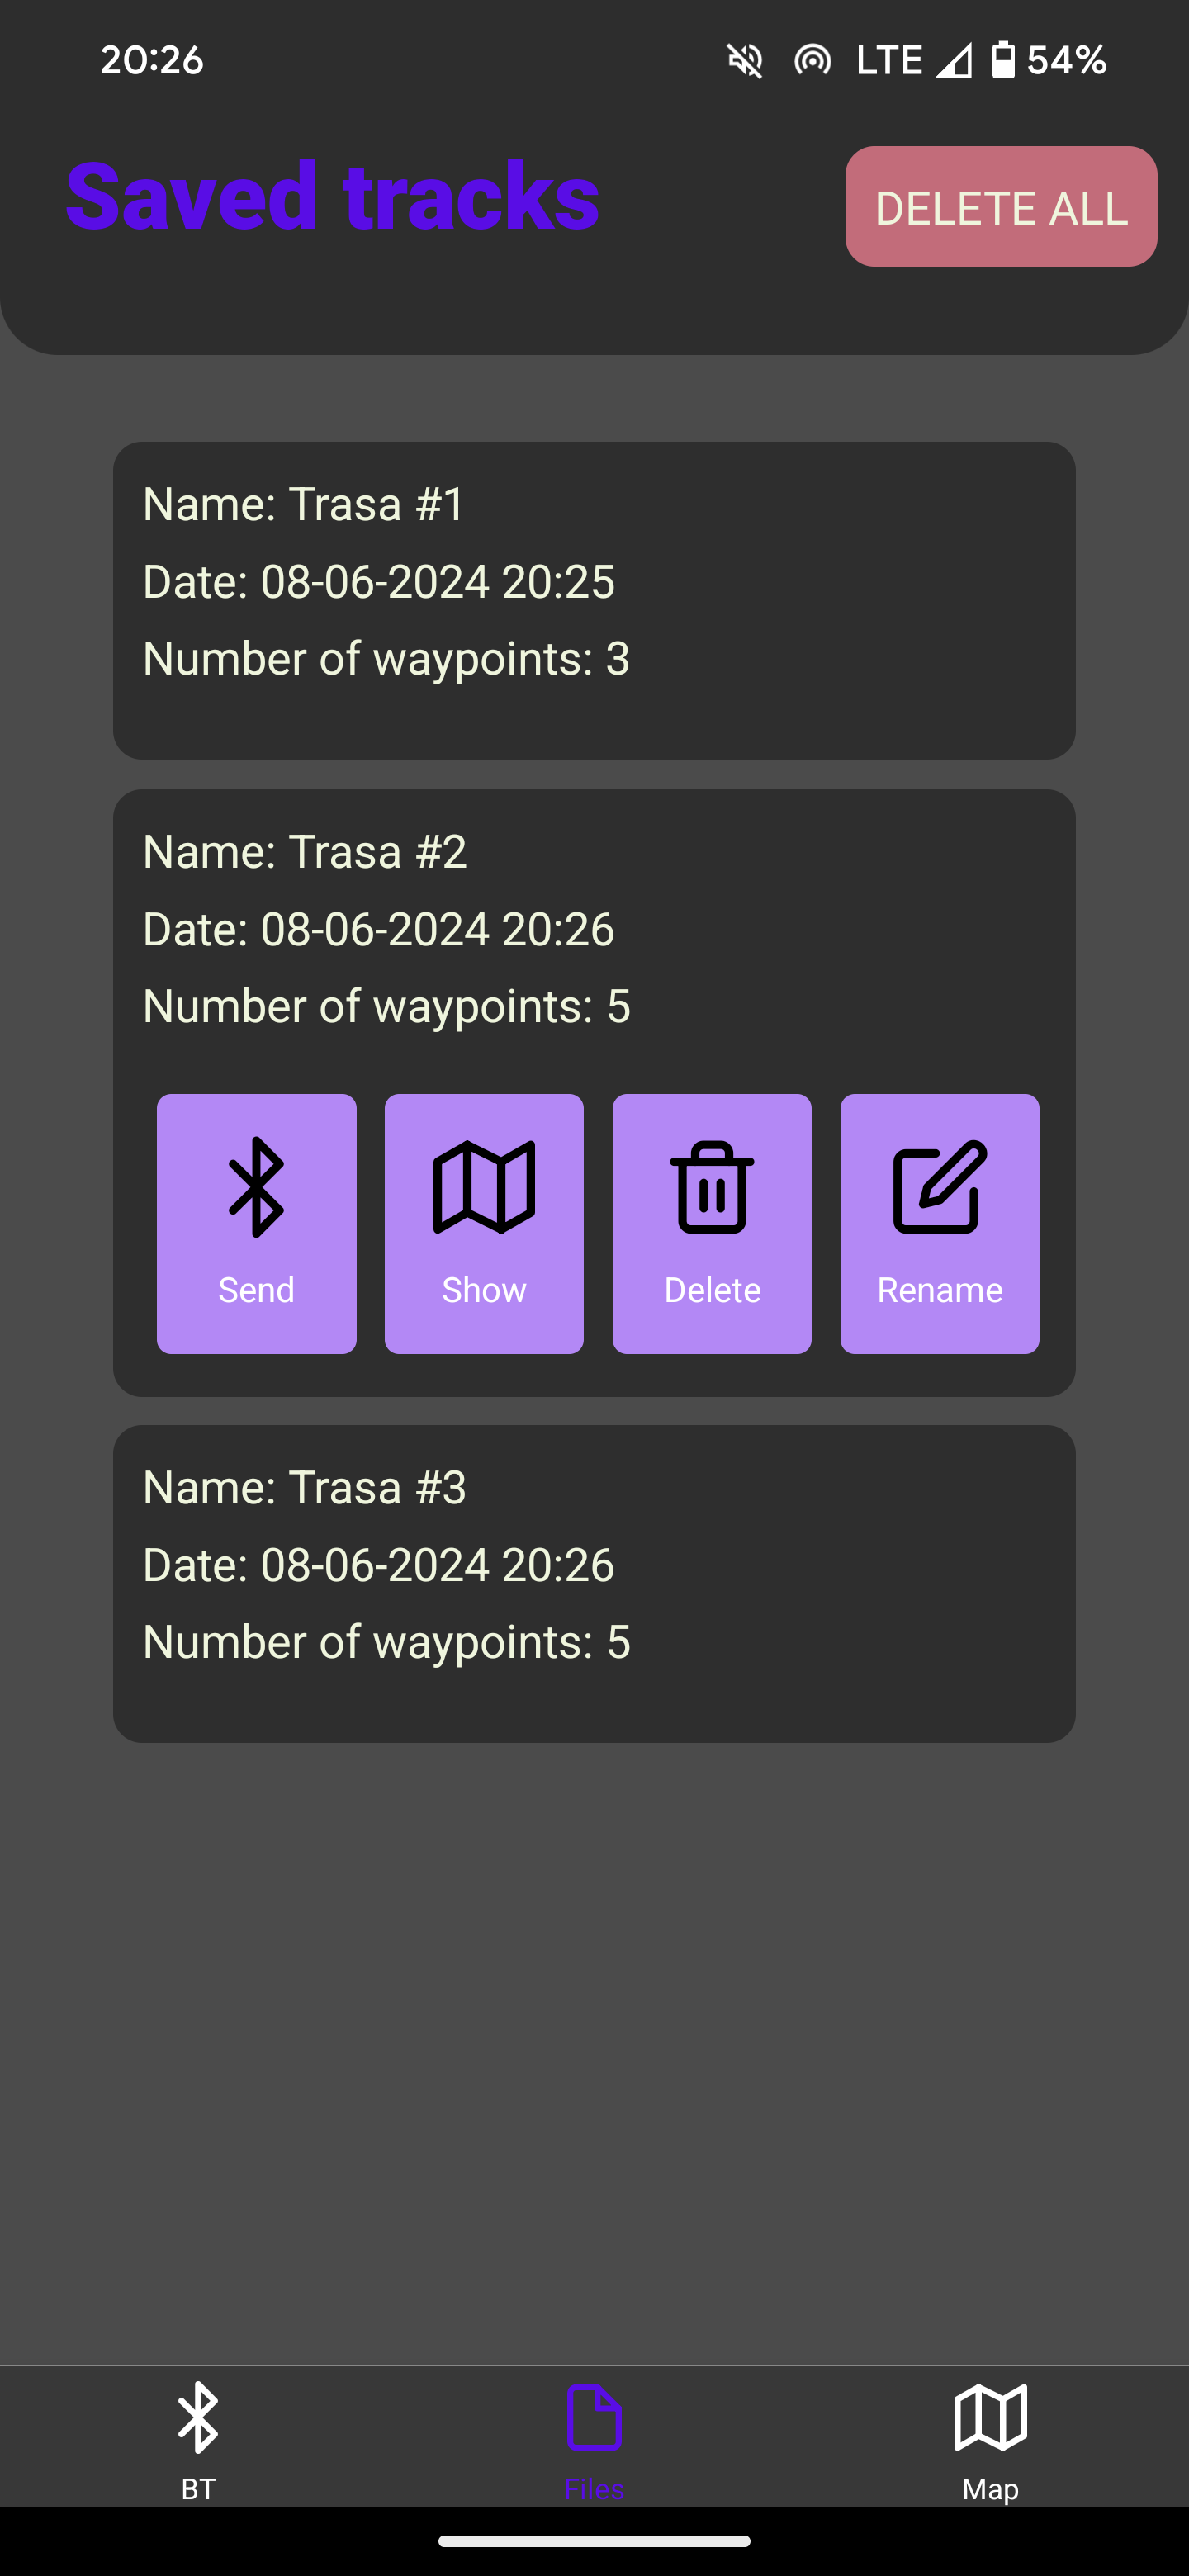
\includegraphics[scale = 0.07]{res/Files.png}
    \caption{Ekran plików}
\end{figure}

Widok ten oferuje możliwość przeglądania zapisanych w urządzeniu tras

Po kliknięciu w trasę, rozwinie się menu z 4 przyciskami:
\begin{itemize}
    \item \textbf{delete} – usuwa wybraną trasę.
    \item \textbf{edit} – przenosi do widoku mapy i wyświetla w nim wybraną trasę pozwalając na jej edycję.
    \item \textbf{send} – pozwala przesłać wybraną trasę do urządzenia SmartCompass jeśli jest ono połączone.
\end{itemize}

\subsubsection{Map}
\begin{figure}[H]
    \centering
    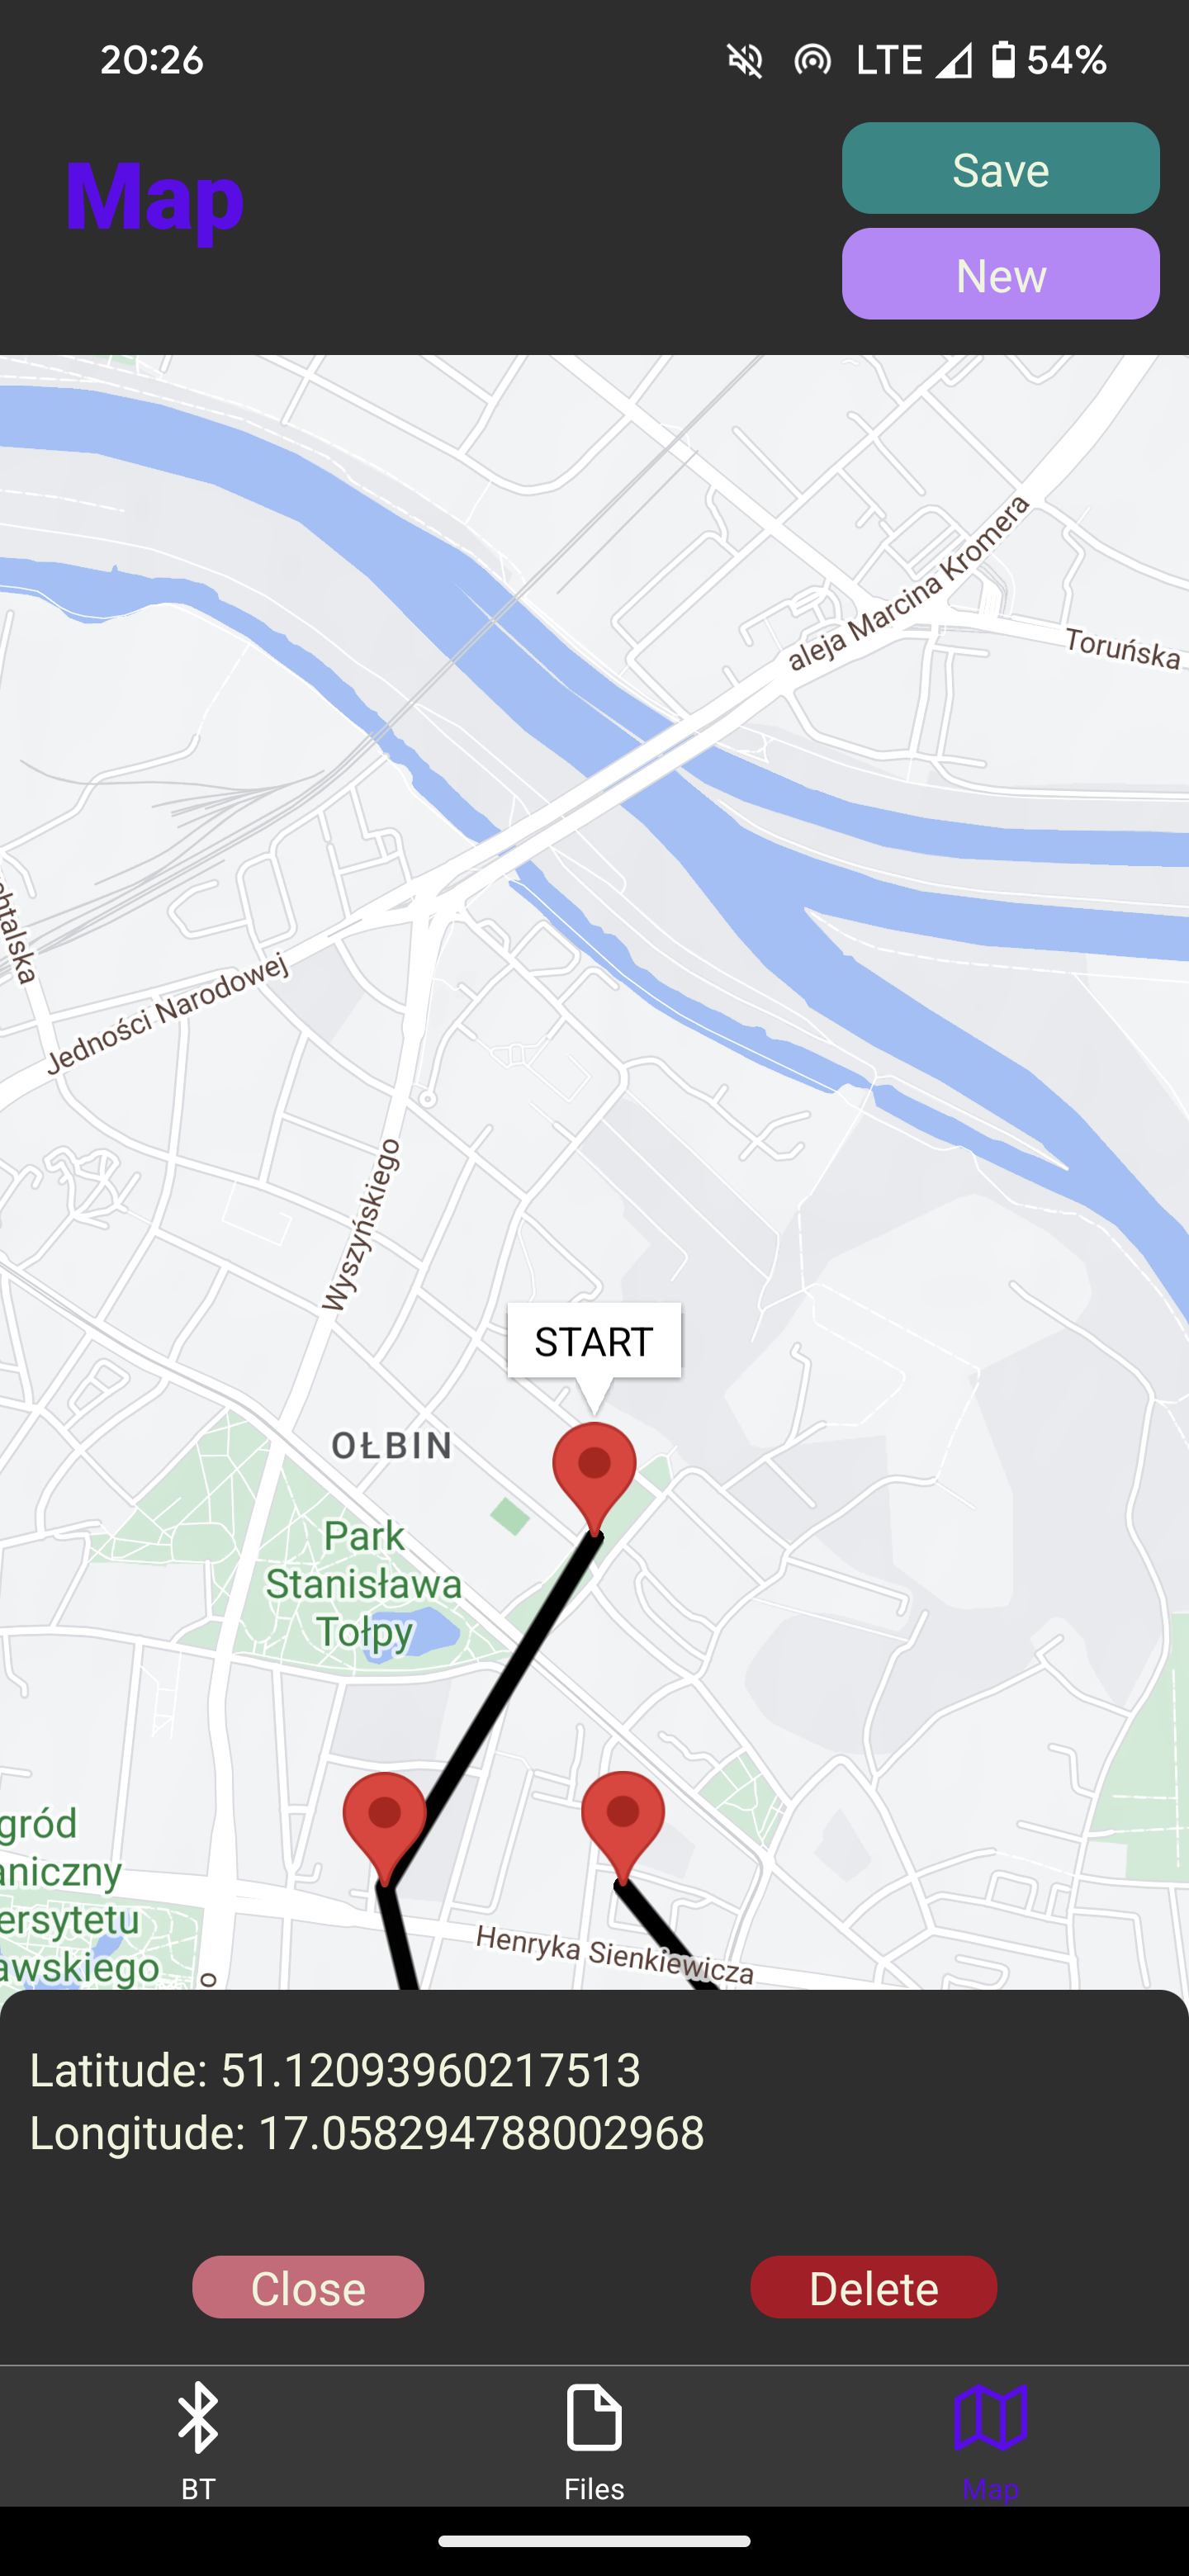
\includegraphics[scale = 0.07]{res/Map.png}
    \caption{Ekran Mapy}
\end{figure}
Widok mapy oferuje możliwość rysowania trasy, dodawania nowej trasy oraz zapisu obecnie narysowanej trasy. W tym celu wykorzystywane są poniższe przyciski:

\begin{itemize}
    \item \textbf{NEW} – wyczyszczenie punktów na mapie, jeśli trasa jest zapisana nie zostanie ona utracona. Pozwala na rysowanie nowej trasy
    \item \textbf{SAVE} – służy do zapisu aktualnie narysowanej trasy. Po kliknięciu pojawi się okienko z miejscem na wpisanie nazwy trasy. Trasa zapisana zostanie do wewnętrznej, statycznej pamięci urządzenia i widoczna będzie w widoku \textbf{Files} po restarcie aplikacji.
\end{itemize}
Ponadto do interakcji z mapą użytkownik wykorzystuje następujące gesty:
\begin{itemize}
    \item \textbf{przytrzymanie palcem w pustym miejscu na mapie} – dodanie nowego punktu
    \item \textbf{dłuższe przytrzymanie znacznika punktu} – przejście w tryb przenoszenia punktu poprzez przesuwanie palcem po ekranie. Znacznik zostanie upuszczony po oderwaniu palca od ekranu
    \item \textbf{kliknięcie w znacznik} – nad znacznikiem wyświetli się małe pole z jego numerem na trasie lub napisem \textit{START/META}. Ponadto na dole ekranu wyświetli się okno z dokładną lokalizacją punktu. Kliknięcie w puste miejsce na mapie spowoduje zamknięcie tego okna i zniknięcie pola nad znacznikiem.
\end{itemize}

\section{Możliwości rozwoju}
\subsection{Rozwój urządzenia}
W aktualnej wersji prototyp spełnia wszystkie wymagania prototypu funkcjonalnego, tzn. pozwala na:
\begin{itemize}
    \item Weryfikacje komunikacji między wszystkimi komponentami.
    \item Weryfikacje działania algorytmu nawigacji.
    \item Weryfikacje działania aplikacji mobilnej.
    \item Sprawdzenie trafności pomysłu na projekt. \textit{(Czy urządzenie w praktyce ma sens?)}
    \item Szybką iterację nad projektem. \textit{(Wymiana modułów i sensorów bez dużych nakładów czasowych i finansowych)}
\end{itemize}
Następnym krokiem w rozwoju urządzenia byłoby przygotowanie produktu do produkcji seryjnej. Wymagałoby to:
\begin{itemize}
    \item Zaprojektowanie dedykowanego układu PCB, który zintegruje wszystkie komponenty i umożliwi miniaturyzacje urządzenia.
    \item Zaprojektowanie dedykowanego modułu zasilania, który będzie spełniał wymagania dotyczące czasu pracy urządzenia.
    \item Zaprojektowanie obudowy, która będzie spełniała wymagania wodoodporności i odporności na wstrząsy.
\end{itemize}
Dodatkowo, w celu zwiększenia atrakcyjności produktu można wprowadzić usprawnienia:
\begin{itemize}
    \item W interfejsie użytkownika - dodanie dodatkowych informacji na wyświetlaczu, prezentacja informacji w bardziej atrakcyjny sposób.
    \item W stabilności działania - poprawa algorytmów nawigacji, zwiększenie dokładności pomiarów.
    \item W zużyciu energii - zastosowanie bardziej energooszczędnych komponentów, optymalizacja algorytmów.
    \item W funkcjonalności - dodanie dodatkowych funkcji, takich jak zapisywanie przebytej trasy, zapisywanie punktów zainteresowania, przechowywanie większej liczby tras.
\end{itemize}

\subsection{Rozwój aplikacji mobilnej}
Aplikacja realizuje zdefiniowane dla niej założenia. Potencjał na rozwój znajduje się w interfejsie użytkownika i, pomimo że jest kompletny, można wprowadzić zmiany, które poprawią ogólne wrażenia oraz intuicyjność korzystania z aplikacji dla użytkownika końcowego.